% !TEX program = xelatex
\documentclass[aspectratio=169,10pt]{ctexbeamer}

\usetheme{hkustgzugod}
\usepackage{amssymb}
\usepackage{amsmath}
\usepackage{booktabs}
\usepackage{tabularx}
\usepackage{adjustbox}
\usepackage{listings}
\usepackage{tikz}
\usetikzlibrary{arrows.meta,positioning,shapes.geometric,fit}
\graphicspath{{figures/}}

\title[RoadGen3D]{RoadGen3D: From Design Intent to Reviewable 3D Street Scenes}
\subtitle{Rule/Constraint-Driven, AI-Assisted Street Scene Generation and Evaluation}
\author[Shiqi Wang · GIStudio]{Shiqi Wang \quad GIStudio}
\institute[HKUST(GZ) UGOD]{HKUST(GZ) Society Hub\\Urban Governance and Design (UGOD)}
\setsource{GIStudio Internal Project}{2026}
\setdomains{\domaintag{Urban Design}\domaintag{3D Generation}\domaintag{GeoAI}}
\setpresenter{Shiqi Wang}
\setvenue{Faculty Project Presentation}
\date{2026-07-10}
\setfigureprefix{Figure}
\renewcommand{\titlemetaline}{%
  \ifdefempty{\presenter}{}{Presenter: \presenter\metasep}%
  \ifdefempty{\presvenue}{}{\presvenue\metasep}%
  \insertdate}

\newcommand{\statusdone}{\tikz[baseline=-0.55ex]\node[rounded corners=2pt,fill=hkustblue2,text=white,inner xsep=4pt,inner ysep=1.5pt,font=\tiny\bfseries]{Implemented};}
\newcommand{\statuspartial}{\tikz[baseline=-0.55ex]\node[rounded corners=2pt,fill=hkustgold,text=white,inner xsep=4pt,inner ysep=1.5pt,font=\tiny\bfseries]{Conditional};}
\newcommand{\statusnext}{\tikz[baseline=-0.55ex]\node[rounded corners=2pt,fill=hkustgrey,text=white,inner xsep=4pt,inner ysep=1.5pt,font=\tiny\bfseries]{Next};}
\newcommand{\sourcefoot}[1]{\vfill{\tiny\color{hkustgrey}Evidence: \texttt{#1}}}
\newcommand{\artifact}[1]{\texttt{\color{hkustblue2}#1}}
\newcommand{\flowarrow}{\tikz[baseline=-0.4ex]\draw[-{Stealth[length=2mm]},line width=0.8pt,color=hkustgold] (0,0)--(0.5,0);}
\newcommand{\smallclaim}[1]{\par\smallskip{\small\color{hkustblue}\bfseries #1}\par}

\lstset{
  basicstyle=\ttfamily\scriptsize,
  keywordstyle=\color{hkustblue}\bfseries,
  stringstyle=\color{hkustgold},
  commentstyle=\color{hkustgrey},
  showstringspaces=false,
  breaklines=true,
  columns=fullflexible,
  frame=single,
  rulecolor=\color{cardgrey},
  backgroundcolor=\color{bgsoft},
  xleftmargin=2mm,
  xrightmargin=2mm
}

\begin{document}

% -----------------------------------------------------------------------------
\begin{frame}[plain]
  \titlepage
\end{frame}

% -----------------------------------------------------------------------------
\begin{frame}{RoadGen3D studies a reviewable generation pipeline, not merely a 3D viewer}
  \small
  \begin{columns}[T,onlytextwidth]
    \column{0.43\textwidth}
      \begin{callout}[One-sentence position]
        A \shl{rule- and constraint-driven, AI-assisted} system for generating and evaluating 3D urban street scenes.
      \end{callout}
      \tightgap
      \begin{itemize}
        \item How does an input become specific roads and facilities?
        \item Which rules pass, and where does a design fail?
        \item Why do alternatives differ, and can they be reproduced?
      \end{itemize}
      \smallclaim{Core contribution path}
      \centering
      \keyword{Design intent} \flowarrow
      \keyword{Explicit IR} \flowarrow
      \keyword{3D artifacts} \flowarrow
      \keyword{Evaluation}
    \column{0.54\textwidth}
      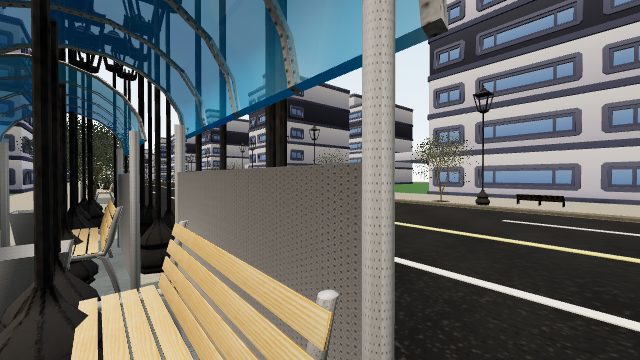
\includegraphics[width=\linewidth,height=0.53\textheight,keepaspectratio]{scene_bus_stop_detail.png}
      \figcap{1}{A semantic edit becomes a bus shelter, seating, road geometry, and building frontage. The image is one form of result evidence.}
  \end{columns}
  \sourcefoot{docs/ROADGEN3D\_FRAMEWORK.md; docs/current-progress.md}
  \note{Do not open with “we built an attractive viewer.” Define the research object as a controllable, traceable, and evaluable generation pipeline.}
\end{frame}

% -----------------------------------------------------------------------------
\begin{frame}[plain,c]{The system compiles design intent into evaluable scenes and retains human review}
  \centering
  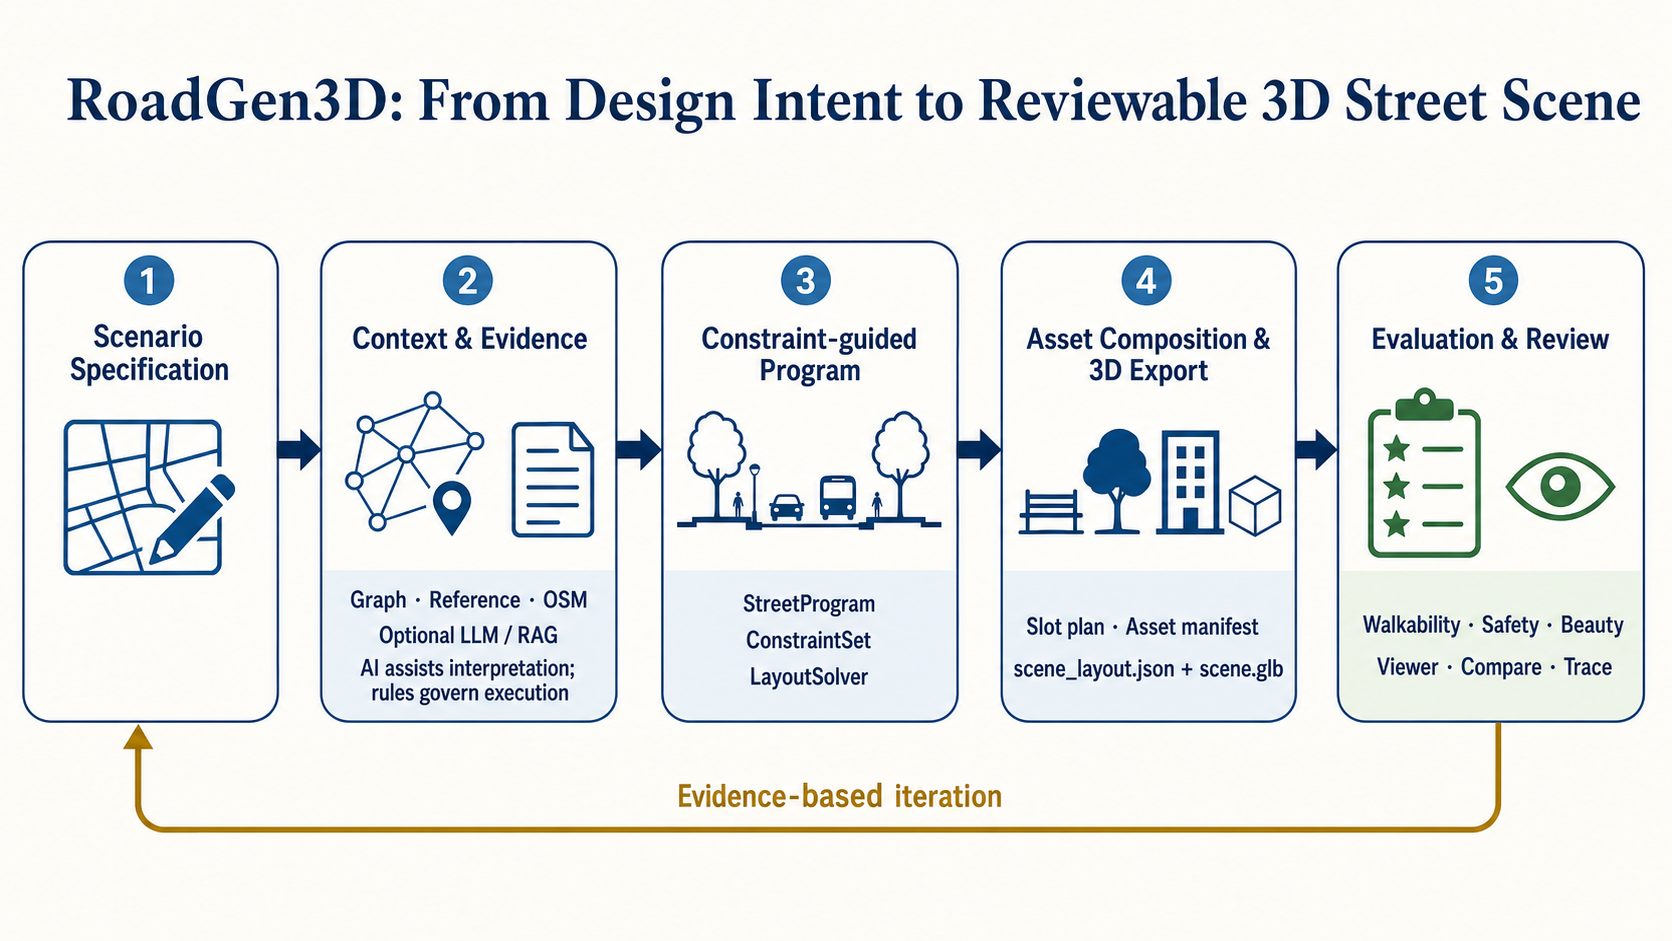
\includegraphics[width=0.97\paperwidth,height=0.70\paperheight,keepaspectratio]{roadgen3d_workflow.png}
  \par\vspace{-1mm}
  {\scriptsize\color{hkustgrey}AI assists interpretation; rules govern execution. Evaluation informs the next scenario iteration rather than creating an unsupervised decision loop.}
  \note{Use 45 seconds to explain five stages: scenario specification, context and evidence, constraint-guided program, assets and export, then evaluation and review.}
\end{frame}

% -----------------------------------------------------------------------------
\begin{frame}{Explicit intermediate representations separate natural language from 3D geometry}
  \begin{columns}[T,onlytextwidth]
    \column{0.59\textwidth}
      \renewcommand{\arraystretch}{1.02}
      \scriptsize
      \begin{tabularx}{\linewidth}{@{}p{0.34\linewidth}X@{}}
        \toprule
        \theadrow \thc{Intermediate representation} & \thc{Question answered} \\
        \midrule
        \artifact{DesignDraft} & What does the user require, and which fields come from explicit input, a preset, or evidence? \\
        \altrow \artifact{SceneContext} & Does the run use a graph template, reference, OSM input, or a compatibility template? \\
        \artifact{StreetProgram} & How are cross-sections, functional bands, demands, and furniture goals represented? \\
        \altrow \artifact{ConstraintSet} & Which requirements are hard rules and which are soft objectives? \\
        \artifact{LayoutSolverResult} & What are the band widths, slot plans, conflicts, and fallbacks? \\
        \altrow \artifact{scene\_layout.json} & Which facts can the Viewer, evaluation, diff, and reproduction workflows share? \\
        \bottomrule
      \end{tabularx}
    \column{0.38\textwidth}
      \small
      \begin{callout}[Why not prompt-to-mesh?]
        Street design must preserve \shl{clear sidewalk width, transit edges, furniture spacing, refuge islands, collision checks, and rule evidence}. A final mesh alone cannot explain these decisions.
      \end{callout}
      \tightgap
      \begin{exampleblock}{Two outputs, distinct roles}
        \begin{itemize}
          \item \artifact{scene.glb}: rendering and interchange
          \item \artifact{scene\_layout.json}: factual and evaluation contract
        \end{itemize}
      \end{exampleblock}
  \end{columns}
  \sourcefoot{docs/DATA\_CONTRACTS.md; src/roadgen3d/services/design\_types.py; src/roadgen3d/types.py}
\end{frame}

% -----------------------------------------------------------------------------
\begin{frame}{AI interprets intent and retrieves evidence; deterministic rules govern execution}
  \footnotesize
  \begin{columns}[T,onlytextwidth]
    \column{0.31\textwidth}
      \begin{block}{AI / RAG support}
        \begin{itemize}
          \item Intent parsing and retrieval queries
          \item PDF / GraphRAG / parameter triples
          \item Parameter suggestions and field-level citations
          \item Optional visual evaluation and recommendations
        \end{itemize}
      \end{block}
    \column{0.31\textwidth}
      \begin{alertblock}{Rules and contracts}
        \begin{itemize}
          \item Compose-patch allowlist
          \item Template-patch validation
          \item Hard and soft constraints
          \item Geometry, collision, and carriageway-intrusion vetoes
        \end{itemize}
      \end{alertblock}
    \column{0.31\textwidth}
      \begin{exampleblock}{Traceable outputs}
        \begin{itemize}
          \item Final values and source priority
          \item Citations and overridden candidates
          \item Requested and used backend
          \item Fallback reasons and warnings
        \end{itemize}
      \end{exampleblock}
  \end{columns}
  \tightgap
  \begin{callout}[Key invariant]
    \shl{Manual and explicit inputs} outrank LLM suggestions. If a learned component or RAG is unavailable, record the fallback; never substitute silently.
  \end{callout}
  \sourcefoot{src/roadgen3d/llm/design\_workflow.py; src/roadgen3d/services/design\_runtime.py; generation\_trace.json}
\end{frame}

% -----------------------------------------------------------------------------
\begin{frame}{The road skeleton bounds the space; the solver compiles demands into slot plans}
  \begin{columns}[T,onlytextwidth]
    \column{0.48\textwidth}
      \begin{block}{1. Graph / Reference Bridge}
        base annotation + \artifact{template\_patch}
        \flowarrow RoadSegmentGraph + PlacementContext
      \end{block}
      \tightgap
      \begin{block}{2. Program + Constraints}
        \artifact{StreetProgram} describes bands, demands, and objectives. \artifact{ConstraintSet} compiles the design rules.
      \end{block}
      \tightgap
      \begin{block}{3. Layout Solver}
        Produces band widths, slot plans, rule evaluations, conflicts, and fallback provenance.
      \end{block}
    \column{0.49\textwidth}
      \begin{tikzpicture}[x=0.68cm,y=0.68cm]
        \fill[bgsoft] (0,0) rectangle (8,5.2);
        \fill[hkustgoldbg] (0.3,0.4) rectangle (1.5,4.8);
        \fill[cardgrey] (1.5,0.4) rectangle (2.5,4.8);
        \fill[hkustblue2!80] (2.5,0.4) rectangle (5.5,4.8);
        \fill[cardgrey] (5.5,0.4) rectangle (6.5,4.8);
        \fill[hkustgoldbg] (6.5,0.4) rectangle (7.7,4.8);
        \draw[white,dashed,line width=1pt] (4,0.5)--(4,4.7);
        \draw[hkustblue,line width=0.8pt] (0.3,0.4) rectangle (7.7,4.8);
        \node[rotate=90,font=\scriptsize\bfseries] at (0.9,2.6) {Frontage};
        \node[rotate=90,font=\scriptsize\bfseries] at (2.0,2.6) {Sidewalk};
        \node[rotate=90,text=white,font=\scriptsize\bfseries] at (3.3,2.6) {Lane};
        \node[rotate=90,text=white,font=\scriptsize\bfseries] at (4.7,2.6) {Lane};
        \node[rotate=90,font=\scriptsize\bfseries] at (6.0,2.6) {Sidewalk};
        \node[rotate=90,font=\scriptsize\bfseries] at (7.1,2.6) {Furniture};
        \foreach \x in {6.8,7.15,7.5}{\fill[hkustteal] (\x,1.0) circle (0.11);}
        \node[anchor=west,font=\tiny,text=hkustgrey] at (0.3,5.05) {Cross-section bands + allowed placement zones};
      \end{tikzpicture}
      \begin{callout}[Example rules]
        Preserve minimum clear sidewalk width; place bus stops only on transit edges; keep seats outside the stopping envelope; prevent assets from entering the carriageway.
      \end{callout}
  \end{columns}
  \sourcefoot{src/roadgen3d/template\_patch.py; graph\_template\_scene\_bridge.py; design\_rules.py; layout\_solver.py}
\end{frame}

% -----------------------------------------------------------------------------
\begin{frame}{Assets are not scattered randomly: demands, retrieval, filtering, and placement jointly determine the result}
  \small
  \begin{columns}[T,onlytextwidth]
    \column{0.32\textwidth}
      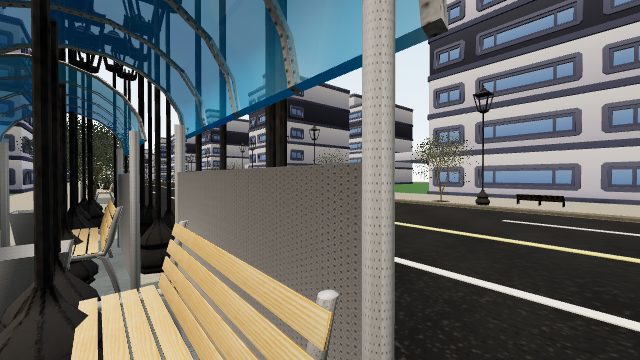
\includegraphics[width=\linewidth]{scene_bus_stop_detail.png}
      \figcap{2}{Human scale: bus shelter and seating}
    \column{0.32\textwidth}
      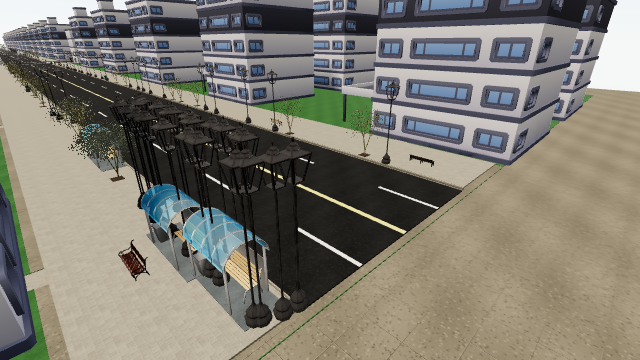
\includegraphics[width=\linewidth]{scene_junction.png}
      \figcap{3}{Overall composition: stops, lights, and buildings}
    \column{0.32\textwidth}
      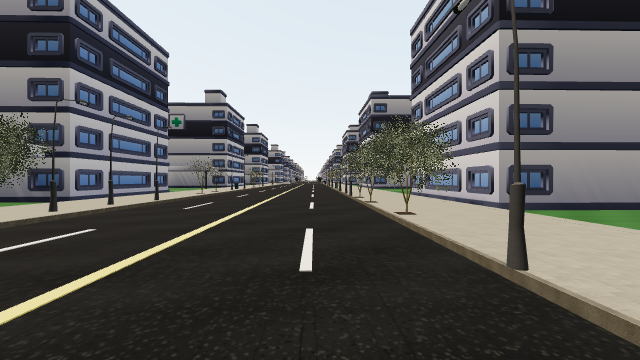
\includegraphics[width=\linewidth]{scene_street.png}
      \figcap{4}{Continuous street frontage}
  \end{columns}
  \tightgap
  \centering
  \keyword{Furniture requirements}
  \flowarrow \keyword{Slot plan}
  \flowarrow \keyword{Manifest retrieval}
  \flowarrow \keyword{Geometry / rule filters}
  \flowarrow \keyword{Placement + mesh export}
  \tightgap
  \begin{callout}[Failure is also data]
    Unplaced assets, collisions, carriageway intrusions, side mismatches, and constraint vetoes remain as diagnostics rather than being forced into the scene.
  \end{callout}
  \sourcefoot{src/roadgen3d/street\_layout.py; placement\_decisions.jsonl; capture\_manifest.json}
\end{frame}

% -----------------------------------------------------------------------------
\begin{frame}{The plan, GLB, and trace jointly form reproducible scene evidence}
  \begin{columns}[T,onlytextwidth]
    \column{0.60\textwidth}
      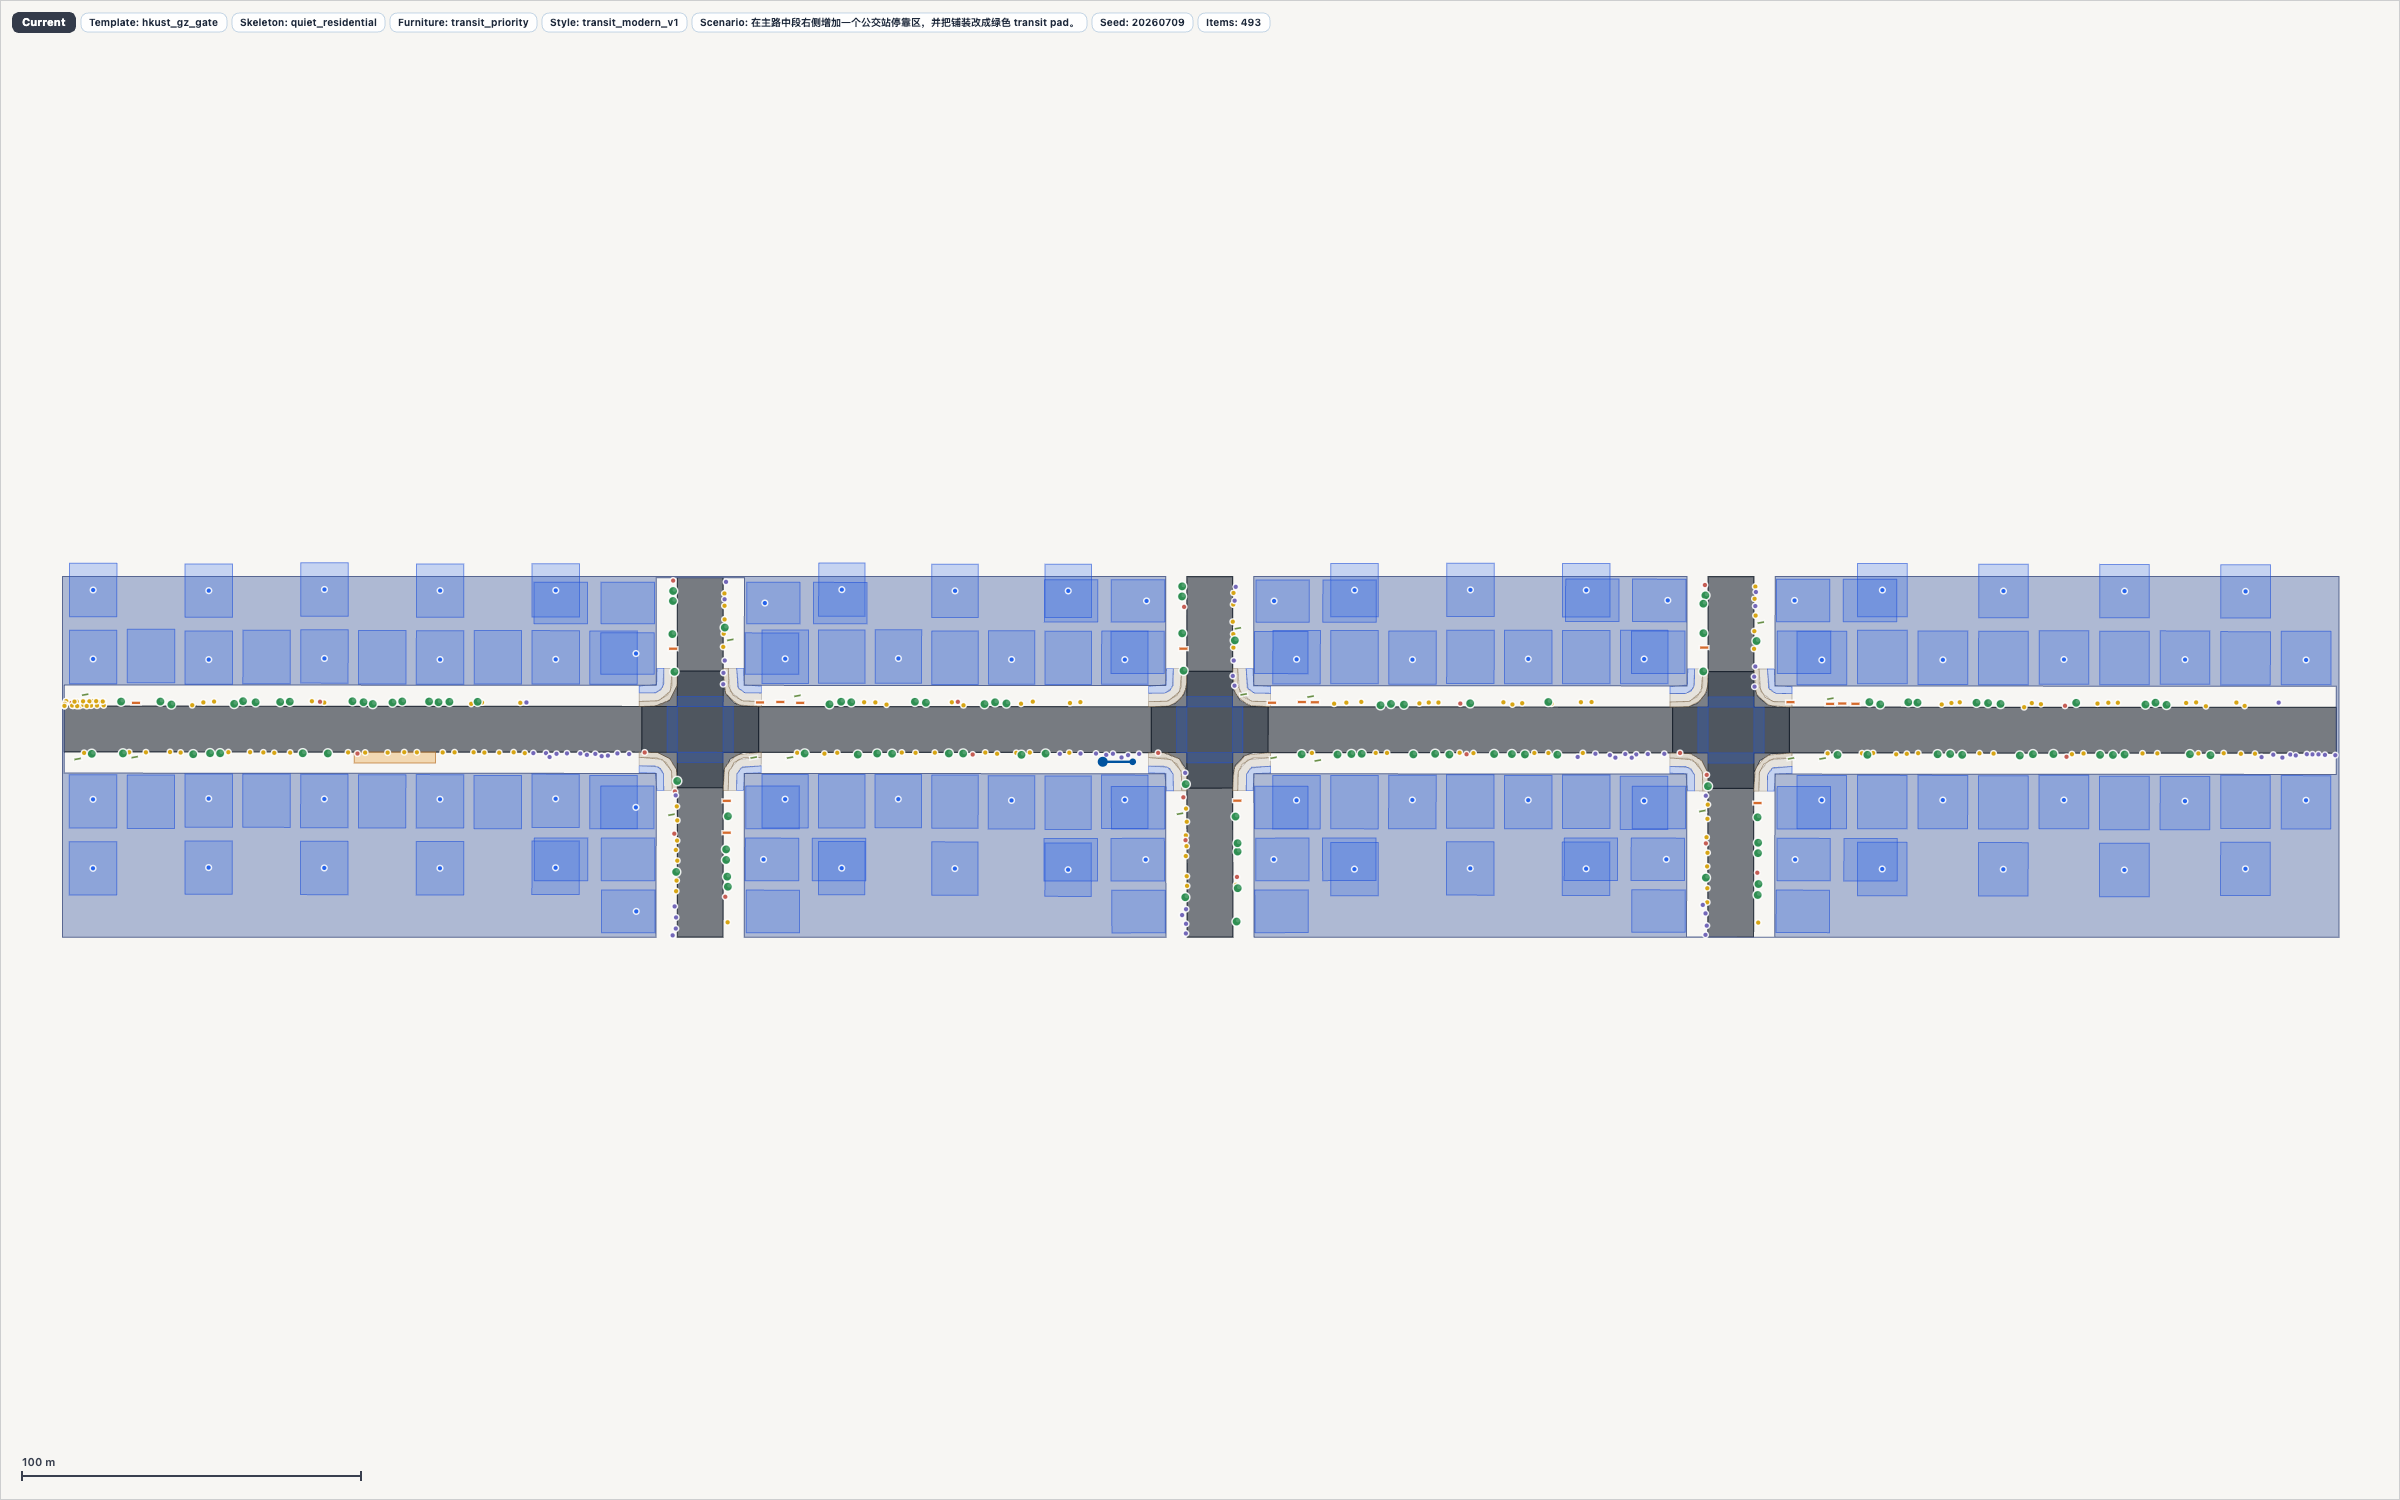
\includegraphics[width=\linewidth,trim=0 450 0 250,clip]{scene_plan_map.png}
      \figcap{5}{Scene Map Plan: roads, surfaces, buildings, and furniture are driven by the same manifest.}
    \column{0.37\textwidth}
      \begin{exampleblock}{Recommended run directory}
        \begin{itemize}
          \item \artifact{scene\_layout.json}
          \item \artifact{scene.glb}
          \item \artifact{generation\_trace.json}
          \item \artifact{production\_steps/}
          \item \artifact{placement\_decisions.jsonl}
          \item \artifact{view\_captures/}
        \end{itemize}
      \end{exampleblock}
      \tightgap
      \begin{callout}[Data authority]
        A GLB can be rebuilt or replaced. Only \shl{layout + provenance} explains where the scene came from.
      \end{callout}
  \end{columns}
  \sourcefoot{artifacts/full\_flow\_smoke/.../20260709T153713Z; web/viewer/src/viewer-api.ts}
\end{frame}

% -----------------------------------------------------------------------------
\begin{frame}{Evaluation separates structural evidence from visual evidence and degrades honestly when inputs are missing}
  \begin{columns}[T,onlytextwidth]
    \column{0.47\textwidth}
      \begin{block}{Structural evidence}
        \artifact{scene\_layout.json}
        \begin{itemize}
          \item Cross-sections and clear widths
          \item Slot, placement, and overlap records
          \item Rule satisfaction, conflicts, and feasibility
          \item Walkability and generation quality
        \end{itemize}
      \end{block}
    \column{0.47\textwidth}
      \begin{exampleblock}{Visual evidence (optional)}
        Rendered views / capture manifest
        \begin{itemize}
          \item Safety and beauty judgments
          \item Multiple views, child view, and overview
          \item LLM status and visual-input status
          \item Scenario-specific rubrics and semantic gates
        \end{itemize}
      \end{exampleblock}
  \end{columns}
  \deckgap
  \begin{callout}[Evaluation integrity]
    Without valid rendered views or an evaluator, Safety, Beauty, and Overall remain \shl{N/A}. Missing evidence is never disguised as a zero or a complete aggregate score.
  \end{callout}
  \sourcefoot{docs/EVALUATION.md; viewer-evaluation-runner.ts; eval\_engine\_ext/road\_metrics}
\end{frame}

% -----------------------------------------------------------------------------
\begin{frame}{A faculty-facing live demo should cover intent, mechanism, result, and evaluation within four minutes}
  \footnotesize
  \begin{columns}[T,onlytextwidth]
    \column{0.60\textwidth}
      \begin{enumerate}
        \item[\textbf{0:00}] \shl{Position}: The Viewer is a review surface. Begin with the final scene and production steps.
        \item[\textbf{0:35}] \shl{Edit}: Enter “Add a 24 m green bus platform on the right side of the arterial's middle segment.”
        \item[\textbf{1:15}] \shl{Compile}: Show the semantic edit, resolved defaults, and validated template patch.
        \item[\textbf{1:55}] \shl{Run}: Submit the job; show monotonic progress, the stage tree, and parameter decisions.
        \item[\textbf{2:40}] \shl{Review}: Load a pre-generated layout; switch among Plan, 3D, and production steps.
        \item[\textbf{3:25}] \shl{Evaluate}: Show metrics, N/A degradation, comparison, and trace.
      \end{enumerate}
    \column{0.37\textwidth}
      \begin{callout}[Preflight]
        \texttt{make api}\\
        \texttt{make viewer-web}\\
        \texttt{GET /api/health}
      \end{callout}
      \tightgap
      \begin{exampleblock}{Contingencies}
        \begin{itemize}
          \item LLM unavailable: \texttt{use\_llm:false}
          \item Slow generation: switch to a pre-generated artifact
          \item Missing visual score: discuss structural evidence only
          \item Job state lost on restart: load the layout from disk
        \end{itemize}
      \end{exampleblock}
  \end{columns}
  \sourcefoot{Makefile; docs/DEPLOYMENT\_AND\_JOBS.md; semantic\_scenario\_edits.py}
\end{frame}

% -----------------------------------------------------------------------------
\begin{frame}{Collaborators integrate through explicit contracts rather than bypassing the IR to edit meshes}
  \renewcommand{\arraystretch}{1.18}
  \begin{adjustbox}{max totalsize={\textwidth}{0.68\textheight},center}
  \begin{tabularx}{\textwidth}{@{}p{0.19\textwidth}p{0.26\textwidth}X p{0.21\textwidth}@{}}
    \toprule
    \theadrow \thc{Role} & \thc{Recommended entry point} & \thc{Primary input / output} & \thc{Boundary to preserve} \\
    \midrule
    Planning / design & Scenario catalog, semantic edit, template patch & scenario intent, functional zones, surface annotations & Do not write meshes directly; validate every patch \\
    \altrow API / application & \texttt{/api/design/draft}, \texttt{/api/scene/jobs} & JSON request, job polling, result / trace & Keep Draft separate from SceneContext \\
    Generation methods & Program, Constraint, Solver, asset backend & IR, slot plan, candidate / placement logs & Record requested / used backend and fallback \\
    \altrow Evaluation / analysis & \texttt{scene\_layout.json}, rendered views & metrics, rubric, comparison, improvement patch & Never fabricate scores without visual evidence \\
    Frontend / external tools & Viewer \texttt{?layout=}, RoadPen bridge & ViewerManifest, GLB, bridge summary / losses & Vite file API is local only; bridge loss must be auditable \\
    \bottomrule
  \end{tabularx}
  \end{adjustbox}
  \sourcefoot{docs/ACTIVE\_ENTRYPOINTS.md; tools/bridge/README.md; web/api/schemas.py}
\end{frame}

% -----------------------------------------------------------------------------
\begin{frame}[fragile]{Minimal API contract: submit a structured job, poll its status, and read the artifacts}
  \begin{columns}[T,onlytextwidth]
    \column{0.56\textwidth}
\begin{lstlisting}[language=bash]
# 1. create
curl -X POST http://127.0.0.1:8010/api/scene/jobs \
  -H 'Content-Type: application/json' \
  --data-binary @scene_job.json
# -> {"job_id":"...", "status":"queued"}

# 2. poll
curl http://127.0.0.1:8010/api/scene/jobs/$JOB_ID
# -> status, stage, progress, operations,
#    result, evaluation, trace
\end{lstlisting}
    \column{0.40\textwidth}
      \begin{block}{Create request}
        \begin{itemize}
          \item \artifact{draft}
          \item \artifact{scene\_context}
          \item \artifact{patch\_overrides}
          \item \artifact{generation\_options}
        \end{itemize}
      \end{block}
      \tightgap
      \begin{exampleblock}{Success result}
        \begin{itemize}
          \item layout / GLB / PLY paths
          \item summary + compose config
          \item viewer URL
          \item generation trace + evaluation
        \end{itemize}
      \end{exampleblock}
  \end{columns}
  \sourcefoot{POST /api/scene/jobs; GET /api/scene/jobs/\{job\_id\}; src/roadgen3d/services/scene\_jobs.py}
\end{frame}

% -----------------------------------------------------------------------------
\begin{frame}{The system demonstrates a controllable generation pipeline, but not yet complete road-engineering capability}
  \small
  \begin{columns}[T,onlytextwidth]
    \column{0.47\textwidth}
      \begin{block}{\statusdone\ Demonstrable now}
        \begin{itemize}
          \item Scenario catalog, semantic edit, and graph templates
          \item Explicit IR, hard / soft rules, and slot solver
          \item Asset retrieval, collision filtering, GLB + layout
          \item Viewer Plan / 3D / compare / history
          \item Structural evaluation, optional visual evaluation, and trace
        \end{itemize}
      \end{block}
    \column{0.47\textwidth}
      \begin{exampleblock}{\statuspartial\ Conditional or experimental}
        \begin{itemize}
          \item LLM, PDF RAG, and GraphRAG require configuration and artifacts
          \item Learned program / placement requires a checkpoint and runtime
          \item Safety / Beauty requires valid visual input
          \item OSM, MetaUrban, and reference paths still need contract convergence
        \end{itemize}
      \end{exampleblock}
  \end{columns}
  \tightgap
  \begin{callout}[\statusnext\ Claims not yet supported]
    Not covered: complete lane movements, signal control, traffic simulation, or production-grade multi-user jobs. Explicit structure alone does not establish a validated neuro-symbolic model.
  \end{callout}
  \sourcefoot{docs/current-progress.md; docs/DEPLOYMENT\_AND\_JOBS.md; docs/ROADGEN3D\_FRAMEWORK.md}
\end{frame}

% -----------------------------------------------------------------------------
\begin{frame}{Validate effectiveness before expanding model and road-engineering complexity}
  \small
  \begin{enumerate}
    \item \shl{Freeze the benchmark and golden artifacts}\par
      Make scenarios, seeds, asset manifests, rendered views, evaluation profiles, and expected results fully reproducible.
    \item \shl{Strengthen road-engineering evaluation}\par
      Add lane connectivity, turn movements, crossing exposure, reachability, delay, and simulation-based safety.
    \item \shl{Reassess the need for learned components}\par
      Raise learned or neuro-symbolic claims only after adding training data, checkpoints, baselines, ablations, and a closed loop with the Viewer.
  \end{enumerate}
  \deckgap
  \begin{callout}[Questions for faculty feedback]
    \begin{itemize}
      \item Which should the first benchmark prioritize: \keyword{rule compliance}, \keyword{design differentiation}, or \keyword{evaluation stability}?
      \item Which interface has the greatest research value: scenario specification, the constraint solver, or the evaluation protocol?
    \end{itemize}
  \end{callout}
  \sourcefoot{README.md Roadmap; docs/EVALUATION.md; docs/current-progress.md}
\end{frame}

% -----------------------------------------------------------------------------
\begin{frame}[plain,c]
  \centering
  {\fontsize{38}{42}\selectfont\bfseries\color{hkustblue} RoadGen3D}
  \deckgap
  {\Large From design intent to \shl{controllable, traceable, and evaluable} 3D street scenes}
  \deckgap
  {\large\color{hkustgrey}Q\,\&\,A}
\end{frame}

% ============================= Appendix =======================================
\appendix

\begin{frame}{Appendix A: Key data contracts and factual outputs}
  \renewcommand{\arraystretch}{1.14}
  \begin{tabularx}{\textwidth}{@{}p{0.25\textwidth}X p{0.22\textwidth}@{}}
    \toprule
    \theadrow \thc{Contract} & \thc{Core content} & \thc{Primary consumer} \\
    \midrule
    \artifact{DesignDraft} & normalized query, config patch, citations, risk, parameter sources & design runtime \\
    \altrow \artifact{SceneContext} & layout mode, graph/reference/OSM, scenario, template patch & context bridge \\
    \artifact{StreetProgram} & cross-section, demands, furniture requirements, objectives & constraint compiler \\
    \altrow \artifact{ConstraintSet} & declarative hard/soft rules, profile, weights & layout solver \\
    \artifact{LayoutSolverResult} & band solution, slot plans, conflicts, fallback provenance & placement / trace \\
    \altrow \artifact{scene\_layout.json} & config, IR, placements, semantic layers, outputs, summary, scene graph & Viewer / evaluation / diff \\
    \bottomrule
  \end{tabularx}
\end{frame}

\begin{frame}{Appendix B: Most important current interfaces}
  \begin{columns}[T,onlytextwidth]
    \column{0.48\textwidth}
      \begin{block}{Generation}
        \begin{itemize}
          \item \texttt{POST /api/design/draft}
          \item \texttt{POST /api/scene/jobs}
          \item \texttt{GET /api/scene/jobs/\{id\}}
          \item \texttt{POST /api/scenario-designs/runs}
          \item \texttt{POST /api/scenario-designs/draft-variant}
        \end{itemize}
      \end{block}
    \column{0.48\textwidth}
      \begin{exampleblock}{Review / Integration}
        \begin{itemize}
          \item \texttt{POST /api/design/evaluate/unified}
          \item \texttt{POST /api/design/evaluate/compare}
          \item \texttt{POST /api/design/capture-views}
          \item Viewer \texttt{?layout=<scene\_layout.json>}
          \item \texttt{tools/bridge/format\_bridge.py}
        \end{itemize}
      \end{exampleblock}
  \end{columns}
  \deckgap
  \begin{callout}[Deployment boundary]
    The most reliable current topology uses HTTP plus an artifact contract on one machine or a shared file system. A remote artifact registry, persistent job table, and worker pool are not yet productionized.
  \end{callout}
\end{frame}

\begin{frame}{Appendix C: Internal invariants worth challenging}
  \begin{enumerate}
    \item \shl{Contract separation}: Compose patches, SceneContext, and generation options remain separate.
    \item \shl{Template immutability}: Patch a deep copy of the base graph; a variant never changes the source template.
    \item \shl{IR before geometry}: Text and LLM outputs never place meshes directly.
    \item \shl{Explainable fallback}: Record the requested backend, used backend, and reason together.
    \item \shl{Placement safety}: Enforce carriageway intrusion, collision, target strip, side, and rule veto checks.
    \item \shl{Visual-score honesty}: Do not return a falsely complete score without visual input.
    \item \shl{Artifact duality}: GLB is the visual carrier; layout is the factual contract.
  \end{enumerate}
\end{frame}

\begin{frame}{Appendix D: Bridge boundaries between RoadPen and RoadGen3D}
  \begin{columns}[T,onlytextwidth]
    \column{0.46\textwidth}
      \begin{block}{Reliably interoperable}
        \begin{itemize}
          \item road topology / centerlines
          \item node coordinates / scale
          \item approximate widths / lane counts
          \item geometry-preserving roundtrip checks
        \end{itemize}
      \end{block}
    \column{0.48\textwidth}
      \begin{exampleblock}{May degrade, but must be recorded explicitly}
        \begin{itemize}
          \item regions / building regions
          \item surface annotations
          \item station strips / junction composition
          \item furniture relationships
          \item warnings, losses, repaired, \texttt{\_\_bridge\_meta}
        \end{itemize}
      \end{exampleblock}
  \end{columns}
  \deckgap
  \begin{callout}[Principle]
    The bridge prioritizes \shl{geometry preservation and auditable semantic degradation}; it does not claim lossless transfer of all semantics.
  \end{callout}
\end{frame}

\end{document}
